\section{Examples of Analytic Solutions of the Forced Golfball Geodesic System}

\subsection{The Boring Golf-Course: $h(q^1,q^2)=0$}
Let us first consider the simplest possible golf-ball course to ensure that the derived model works. That is, let us consider a perfectly flat golfball course, characterized by the height equation $h(x,y)=0$. If our height is zero, then it is immediately clear that our metric $G$ becomes the identity matrix $I$, also known as the kronecker-delta tensor, where the indices of the metric are characterized by $G_{ij}=\delta_{ij}$. In this case, our system of equations derived from \ref{finalgeoeqrearranged} becomes
\begin{align}
v^1 &= \dot{q}^1 \\
v^2 &= \dot{q}^2 \\
\dot{v}^1 &= 0 \\
\dot{v}^2 &= 0
\end{align}

For initial conditions of the golf ball $(q^1_0,q^2_0,v^1_0,v^2_0)$, this describes uniform motion in both $q^1$ and $q^2$ directions, as expected for unconstrained motion on a flat surface with no external forces acting in the plane. Solving the system of differential equations, we achieve

\begin{equation}    
	q^1(t)=v^1_0t + q^1_0, \qquad q^2(t) = v^2_0t + q^2_0, 
\end{equation}

which describes straight line motion on the plane starting at our initial position, as demonstrated in the figure below.


\begin{figure}[H]
	\centering
	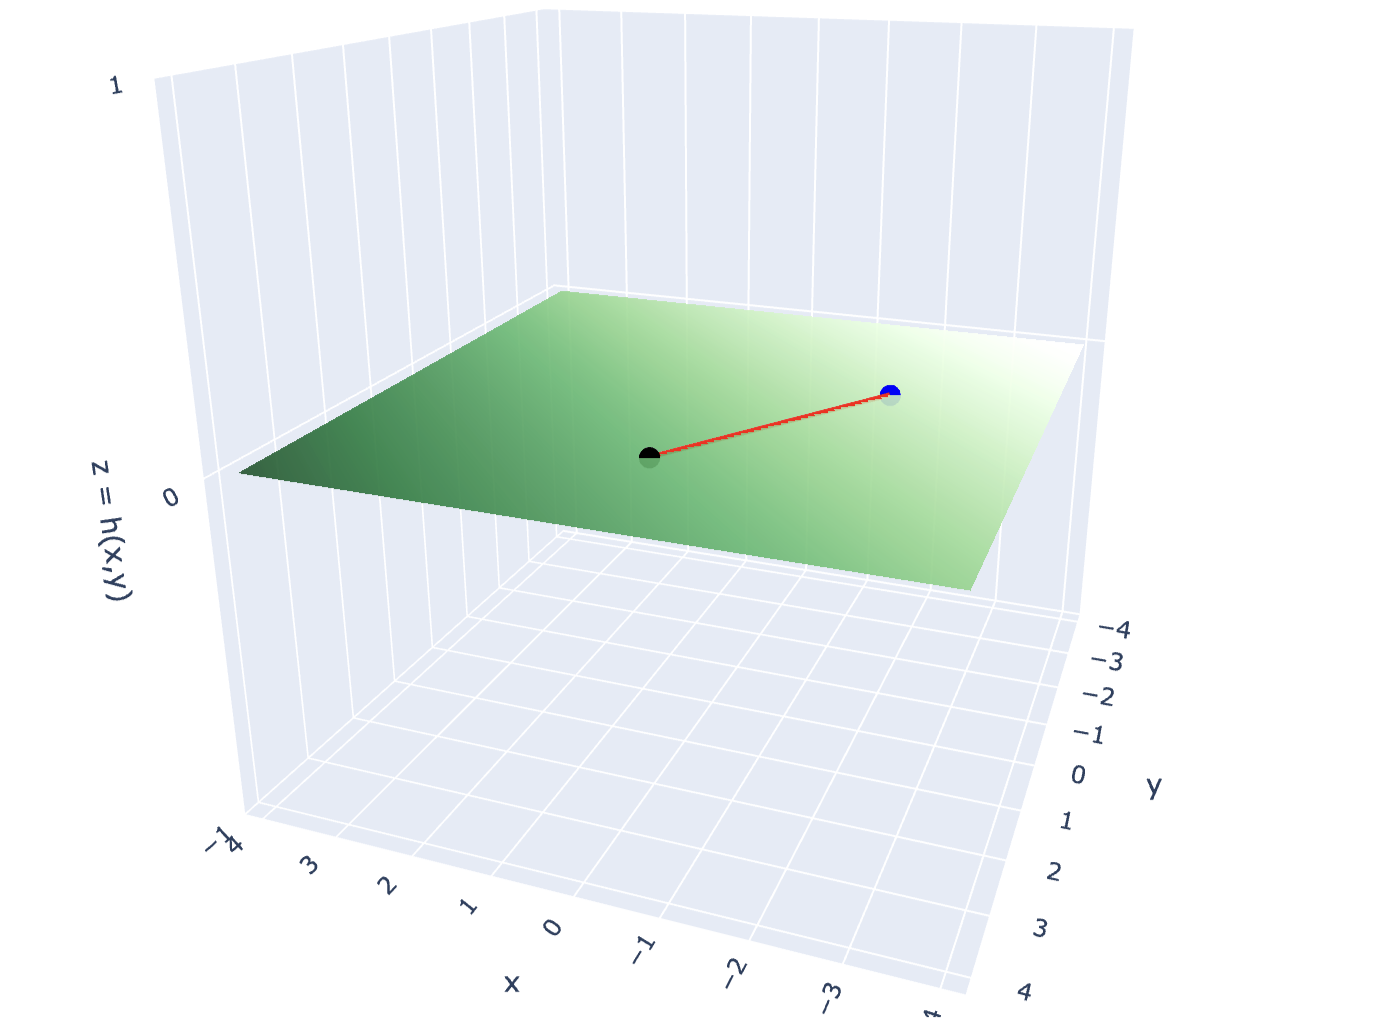
\includegraphics[width=0.55\textwidth]{assets/flat_course.png}
	\caption{Diagram demonstrating the trajectory of a golfball on a flat course. Notice that the ball exhibits straight line motion.}
	\label{fig:course1}
	% Source: https://en.wikiversity.org/wiki/Continuum_mechanics/Calculus_of_variations
\end{figure}

So far, the model is consistent with the observed results. Let us now examine a slightly more complex example.

\subsection{A Slightly Less-Boring Golf Course: $h(q^1,q^2)=\alpha q^1 + \beta q^2$}

Let us now consider the example of a "tilted" golf course. That is, let us describe the golf course as an inclined plane $h(q^1, q^2) = \alpha q^1 + \beta q^2$. Since the expression of the height field is first order in $q^1$ and $q^2$, all second derivatives vanish, yielding a constant metric $G$, namely
\begin{equation}
	G = \begin{pmatrix}
1 + \alpha^2 & \alpha\beta \\
\alpha\beta & 1 + \beta^2
\end{pmatrix}.
\end{equation}
Since the metric itself is constant, so it its inverse $G^{-1}$. Since christoffel symbols function on the derivatives of the entries of the metric $G$, all Christoffel symbols are likewise zero, reducing our equations of motion to a very simple second order ODE, e.g.

\begin{equation}
	\ddot{q}^i = -g G^{ij} \partial_j h.
\end{equation}

Since $h(q^1,q^2)=\alpha q^1 + \beta q^2$, the partial derivatives $\partial_1 h = \alpha$, $\partial_2 h = \beta$ Let $A^i = g G^{i1} \alpha + g G^{i2} \beta$ (note also that $G^{ij}$ is the inverse metric). This reduces our equations of motion for the golfball to a simple constant vector acceleration model, that is

\begin{equation}
	\ddot{q}^i = -A^i \implies \begin{pmatrix}
		\ddot q^1 \\ \ddot q^2
	\end{pmatrix} = -\begin{pmatrix}
		A^1 \\ A^2
	\end{pmatrix}
\end{equation}
which is a constant acceleration in both directions. The general solution is therefore

\begin{equation}
	q^i(t) = q^i_0 + v^i_0 t - \frac{1}{2} A^i t^2,
\end{equation}

or, more explicitly in vector notation,
\begin{equation}
\begin{pmatrix}
q^1(t) \\
q^2(t)
\end{pmatrix}
=
\begin{pmatrix}
q^1_0 \\
q^2_0
\end{pmatrix}
+
\begin{pmatrix}
v^1_0 \\
v^2_0
\end{pmatrix} t
-
\frac{1}{2}
\begin{pmatrix}
A^1 \\
A^2
\end{pmatrix}
t^2
\end{equation}


where
\[
\begin{pmatrix}
A^1 \\
A^2
\end{pmatrix}
=
g G^{-1}
\begin{pmatrix}
\alpha \\
\beta
\end{pmatrix}
\]

This describes a parabola in the $(q^1, q^2)$ plane, rotated according to the slope $(\alpha, \beta)$ of the surface. The trajectory is the projection of uniform acceleration down the gradient of the plane, as expected. Below is a diagram of this exact behavior when the ODE is solved numerically for the given height field. In the example the height field has parameters $\alpha = 0.2, \beta = 0.2$.

\begin{figure}[H]
	\centering
	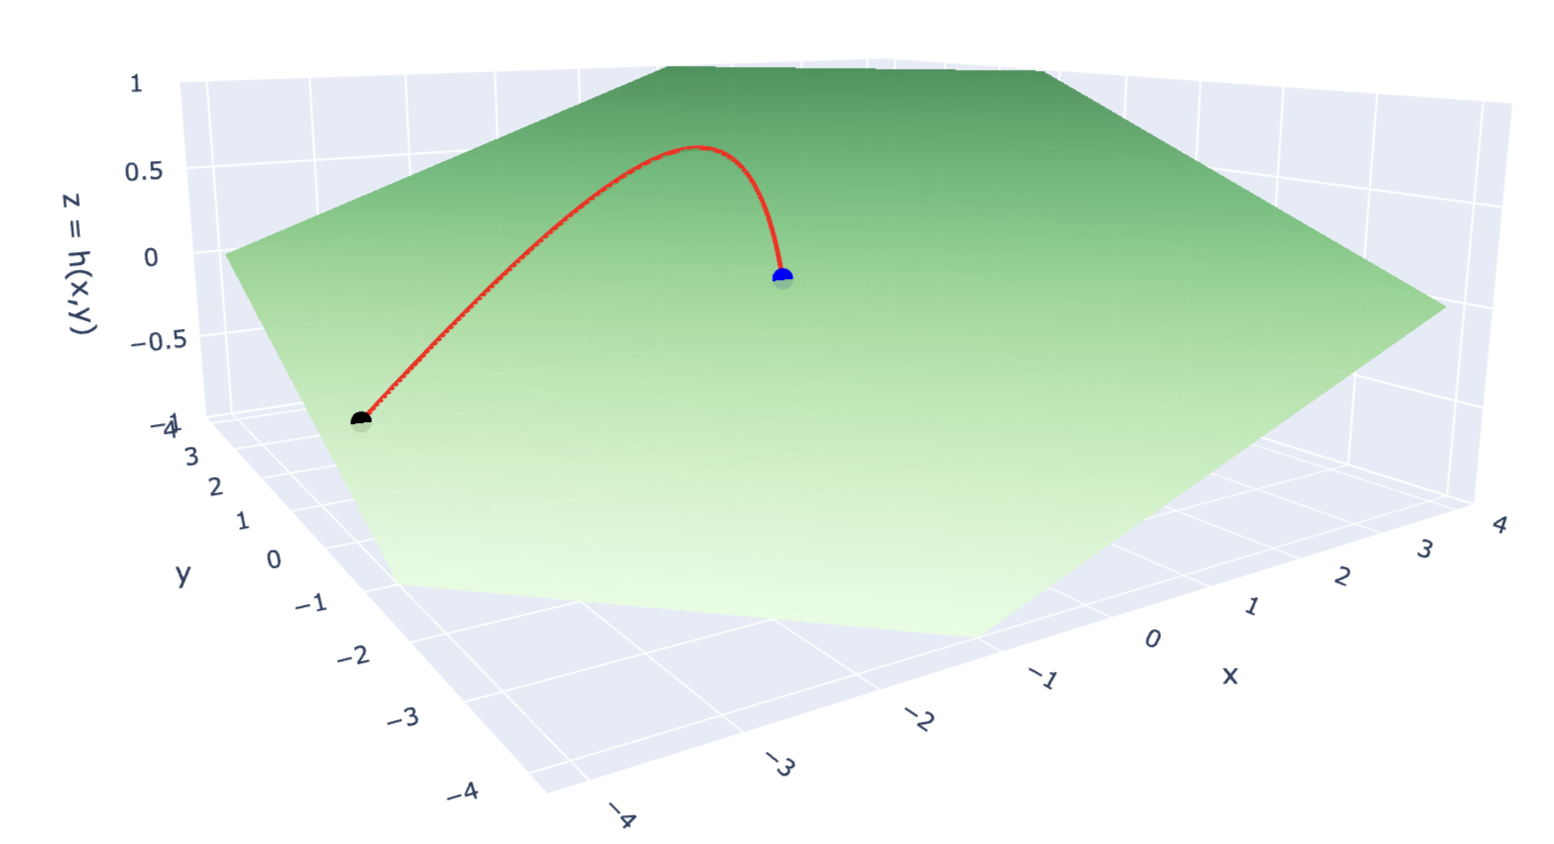
\includegraphics[width=0.55\textwidth]{assets/tilted_course.png}
	\caption{Diagram demonstrating the trajectory of a golfball on a titled plane $h(q^1,q^2)=0.2 q^1 + 0.2 q^2$. Notice that the ball exhibits a rotated parabolic path.}
	\label{fig:course2}
\end{figure}

For more complex course geometries, of which there are many, the Christoffel symbols no longer reduce to zero (indicative of some further local curvature), greatly complicating the computation process of the analytic trajectory expression. While some cases may be possible, it is often more practical in the real world to make very refined estimates using \textbf{numerical methods}, which are commonplace for physicists and computational mathematicians seeking to understand the behavior or more complex dynamical systems or systems of DEs. To reap the full benefits of this abstract minigolf model, let us now consider some more abstract course geometries which may tell us some more insightful things about how particles move on specific geometries when subject to specific forces, for now in a solely qualitative manner.

